\documentclass[11pt]{article}
\usepackage[english]{babel}
\usepackage{amsmath, amsthm, amssymb, mathtools, thmtools, mathdots, tikz, mathrsfs}
%\usepackage{enumerate} conflicts with enumitem
\mathtoolsset{showonlyrefs}
\usepackage[shortlabels]{enumitem}
\usepackage{subcaption}
\usepackage{fancyhdr}
\usepackage{graphicx}
\usepackage{hyperref}
%\usepackage{parskip}
\usepackage[left=1in,top=1in,right=1in,bottom=1in]{geometry}
%\setlength{\headheight}{15.2pt}
%\setlength{\parindent}{0pt}
%\setlength{\parskip}{5pt}
\usepackage{indentfirst}
\newcommand{\eat}[1]{}

%\usetikzlibrary{positioning,matrix}

\hypersetup{colorlinks=true,linkcolor=blue,citecolor=gray}
\addto\extrasenglish{
    \renewcommand{\sectionautorefname}{Section}
    \renewcommand{\subsectionautorefname}{Section}
    \renewcommand{\subsubsectionautorefname}{Section}
}
% comment out the outer \addto\extrasenglish braces if not using babel package



%%%%%%%%%%%%%%%%%%%%%%%%%%%%%%%%%%%%%%%%%%%%%%%%%%%%%%%%%%%%%%%%%%%%%
\declaretheoremstyle[
    shaded={rulecolor={rgb}{0,0,0}, rulewidth=0.5pt, bgcolor={rgb}{1,1,1}}
]{boxedstyle}

\declaretheorem[name={Theorem}, style=boxedstyle, numberwithin=section]{thm}
\declaretheorem[name={Lemma}, style=boxedstyle, sibling=thm]{lem}
\declaretheorem[name={Proposition}, style=boxedstyle, sibling=thm]{prop}
\declaretheorem[name={Corollary}, style=boxedstyle, sibling=thm]{cor}
\declaretheorem[name={Problem}, sibling=thm]{prob}
\declaretheorem[name={Definition}, style=definition, sibling=thm, qed=$\blacksquare$]{df}
\declaretheorem[name={Example}, style=definition, sibling=thm, qed=$\blacksquare$]{example}

%%%%%%%%%%%%%%%%%%%%%%%%%%%%%%%%%%%%%%%%%%%%%%%%%%%%%%%%%%%%%%%%%%%%%

\title{CS 294 Checkpoint 1:\\Variational Auto-encoders and other Generative Models}
\date{26 September 2016}
\author{Project members: Jianbo Chen\quad Billy Fang\quad Cheng Ju}

%%%%%%%%%%%%%%%%%%%%%%%%%%%%%%%%%%%%%%%%%%%%%%%%%%%%%%%%%%%%%%%%%%%%%

%\fancyhf{}
%\fancyhf[HL]{\sc{Billy Fang}}
%\fancyhf[HR]{\rightmark}
%\fancyhf[FC]{\thepage}

%%%%%%%%%%%%%%%%%%%%%%%%%%%%%%%%%%%%%%%%%%%%%%%%%%%%%%%%%%%%%%%%%%%%%
%\newcommand{\m}[1]{\mathcal{#1}}
%\renewcommand{\b}[1]{\mathbb{#1}}
\DeclarePairedDelimiter{\parens}{(}{)}
\DeclarePairedDelimiter{\braces}{\{}{\}}
\DeclarePairedDelimiter{\brackets}{[}{]}
\DeclarePairedDelimiter{\abs}{|}{|}
\DeclarePairedDelimiter{\norm}{\|}{\|}
\DeclarePairedDelimiter{\ceil}{\lceil}{\rceil}
\DeclarePairedDelimiter{\floor}{\lfloor}{\rfloor}
\DeclarePairedDelimiter{\inner}{\langle}{\rangle}
\DeclareMathOperator*{\argmin}{\arg\!\min}
\DeclareMathOperator*{\argmax}{\arg\!\max}
%\DeclareMathOperator{\im}{im}
%\DeclareMathOperator{\Aut}{Aut}
%\DeclareMathOperator{\Inn}{Inn}
%\DeclareMathOperator{\lcm}{lcm}
%\DeclareMathOperator{\trace}{trace}
%\DeclareMathOperator{\Hom}{Hom}
\newcommand{\op}[1]{\operatorname{#1}}
\renewcommand{\b}[1]{\boldsymbol{\mathbf{#1}}}
\renewcommand{\bar}[1]{\overline{#1}}
\renewcommand{\hat}[1]{\widehat{#1}}
\renewcommand{\tilde}[1]{\widetilde{#1}}
\newcommand{\E}{\mathbb{E}}
\renewcommand{\P}{\mathbb{P}}
\newcommand{\Var}{\op{Var}}
\newcommand{\Cov}{\op{Cov}}
\newcommand{\R}{\mathbb{R}}
\newcommand{\N}{\mathbb{N}}
\newcommand{\indep}{\mathop{\rotatebox[origin=c]{90}{$\models$}}}

%%%%%%%%%%%%%%%%%%%%%%%%%%%%%%%%%%%%%%%%%%%%%%%%%%%%%%%%%%%%%%%%%%%%%

%\renewcommand{\familydefault}{\sfdefault}
\DeclareTextFontCommand{\emph}{\bfseries}
%\usepackage{mathptmx}
%\renewcommand{\rmdefault}{ptm}
%\usepackage[default,scale=0.9]{opensans}

\allowdisplaybreaks[1]
\sloppy

%%%%%%%%%%%%%%%%%%%%%%%%%%%%%%%%%%%%%%%%%%%%%%%%%%%%%%%%%%%%%%%%%%%%%


\begin{document}

\maketitle


\section*{Team members and roles}

\begin{itemize}
    \item Jianbo Chen: variational auto-encoder, overall infrastructure
    \item Billy Fang: conditional variational auto-encoder, semi-supervised learning model
    \item Cheng Ju: DRAW (generation with attention models)
\end{itemize}

\section*{Problem statement and background}

Variational auto-encoders (VAEs) \cite{kingma2013auto} are a class of deep generative models based on a variational method in Bayesian inference. There exist many variants including conditional VAEs \cite{doersch2016tutorial}, VAEs tailored for semi-supervised learning \cite{DBLP:journals/corr/KingmaRMW14}, attention-based generative models \cite{gregor2015draw}, and more.

One obvious feature of generative models is their ability to produce realistic images and other output. With sophisticated models, one can even replicate consistent ``style.'' For example, DRAW \cite{gregor2015draw} was able to generate images of house numbers with number combinations not seen in the training set, but with a consistent style/color/font of street sign in each image. Additionally, as models learn to generate realistic output, they learn important features along the way, which potentially can be used for classification; we consider this in the conditional VAE and semi-supervised learning models.

As we implement known models, we also explore generalizations and modifications. We have considered modifying the architecture of the various networks, modifying the various ways one can incorporate side data in the conditional VAE and semi-supervised settings, as well as considering non-isotropic Gaussian models (which the current literature eludes).

Since we are currently at an implementation/exploratory stage, we have not rigorously evaluated the quality of our generated output, but we intend to be more quantitative in this regard later on.

\section*{Data source}

Currently we are using the MNIST handwriting dataset through TensorFlow. We hope to move on to natural images in the future.

\section*{Models}

\begin{enumerate}
    \item \emph{Variational auto-encoder (VAE).} We start from the model used in \cite{kingma2013auto}. We have implemented two types of variational auto-encoder:
    \begin{enumerate}
        \item Baseline model: The first VAE uses single-layer networks for both the encoder and the decoder, which we call fc-VAE. The following is a sample of some of the generated images.
        \item Convolutional model: The second VAE uses convolutional networks for the encoder and  uses deconv nets for the decoder, which we call conv-VAE. A sample of the generated images appears below. Concretely, our encoder is of the form:
        \[\text{conv-BN-ReLU-conv-BN-ReLU-linear-BN-ReLU}.\]
        The decoder is of the form:
        \[\text{Linear-ReLU-deconv-BN-ReLU-deconv-BN-RelU}.\]
    \end{enumerate}
    \begin{figure}[!ht]
        \centering
        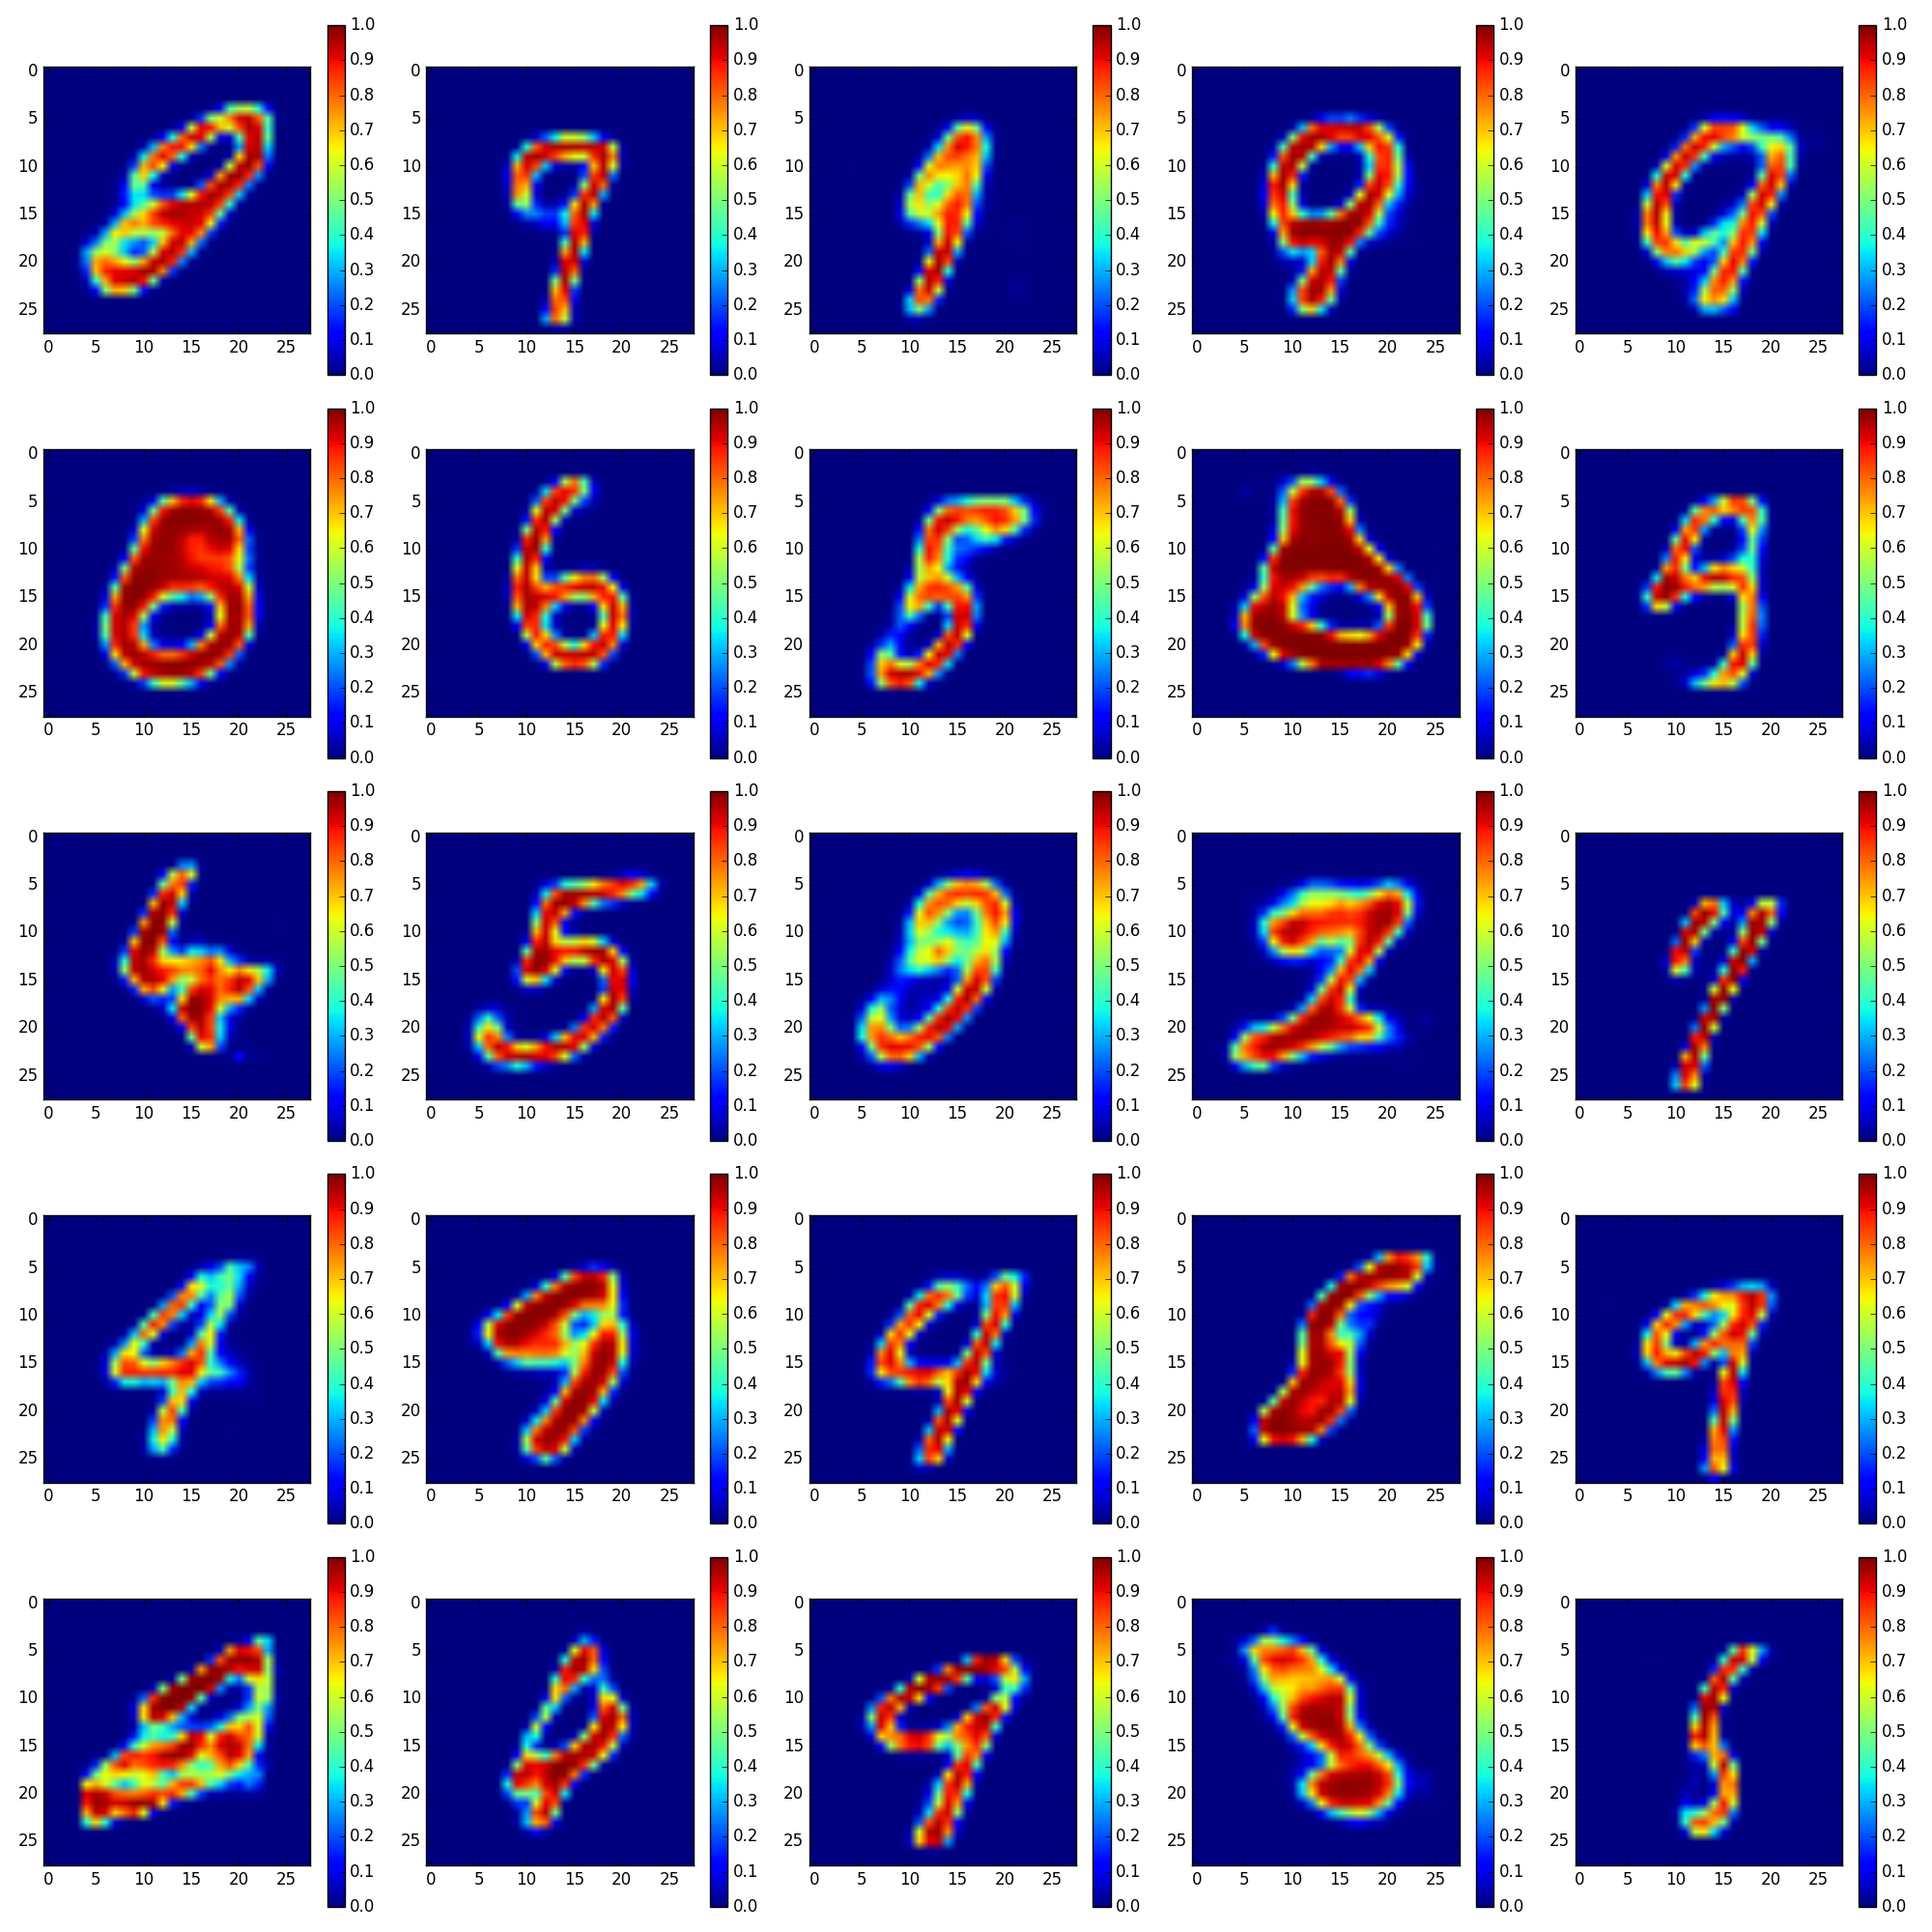
\includegraphics[width=0.4\textwidth]{img/fcvae.png}\quad
        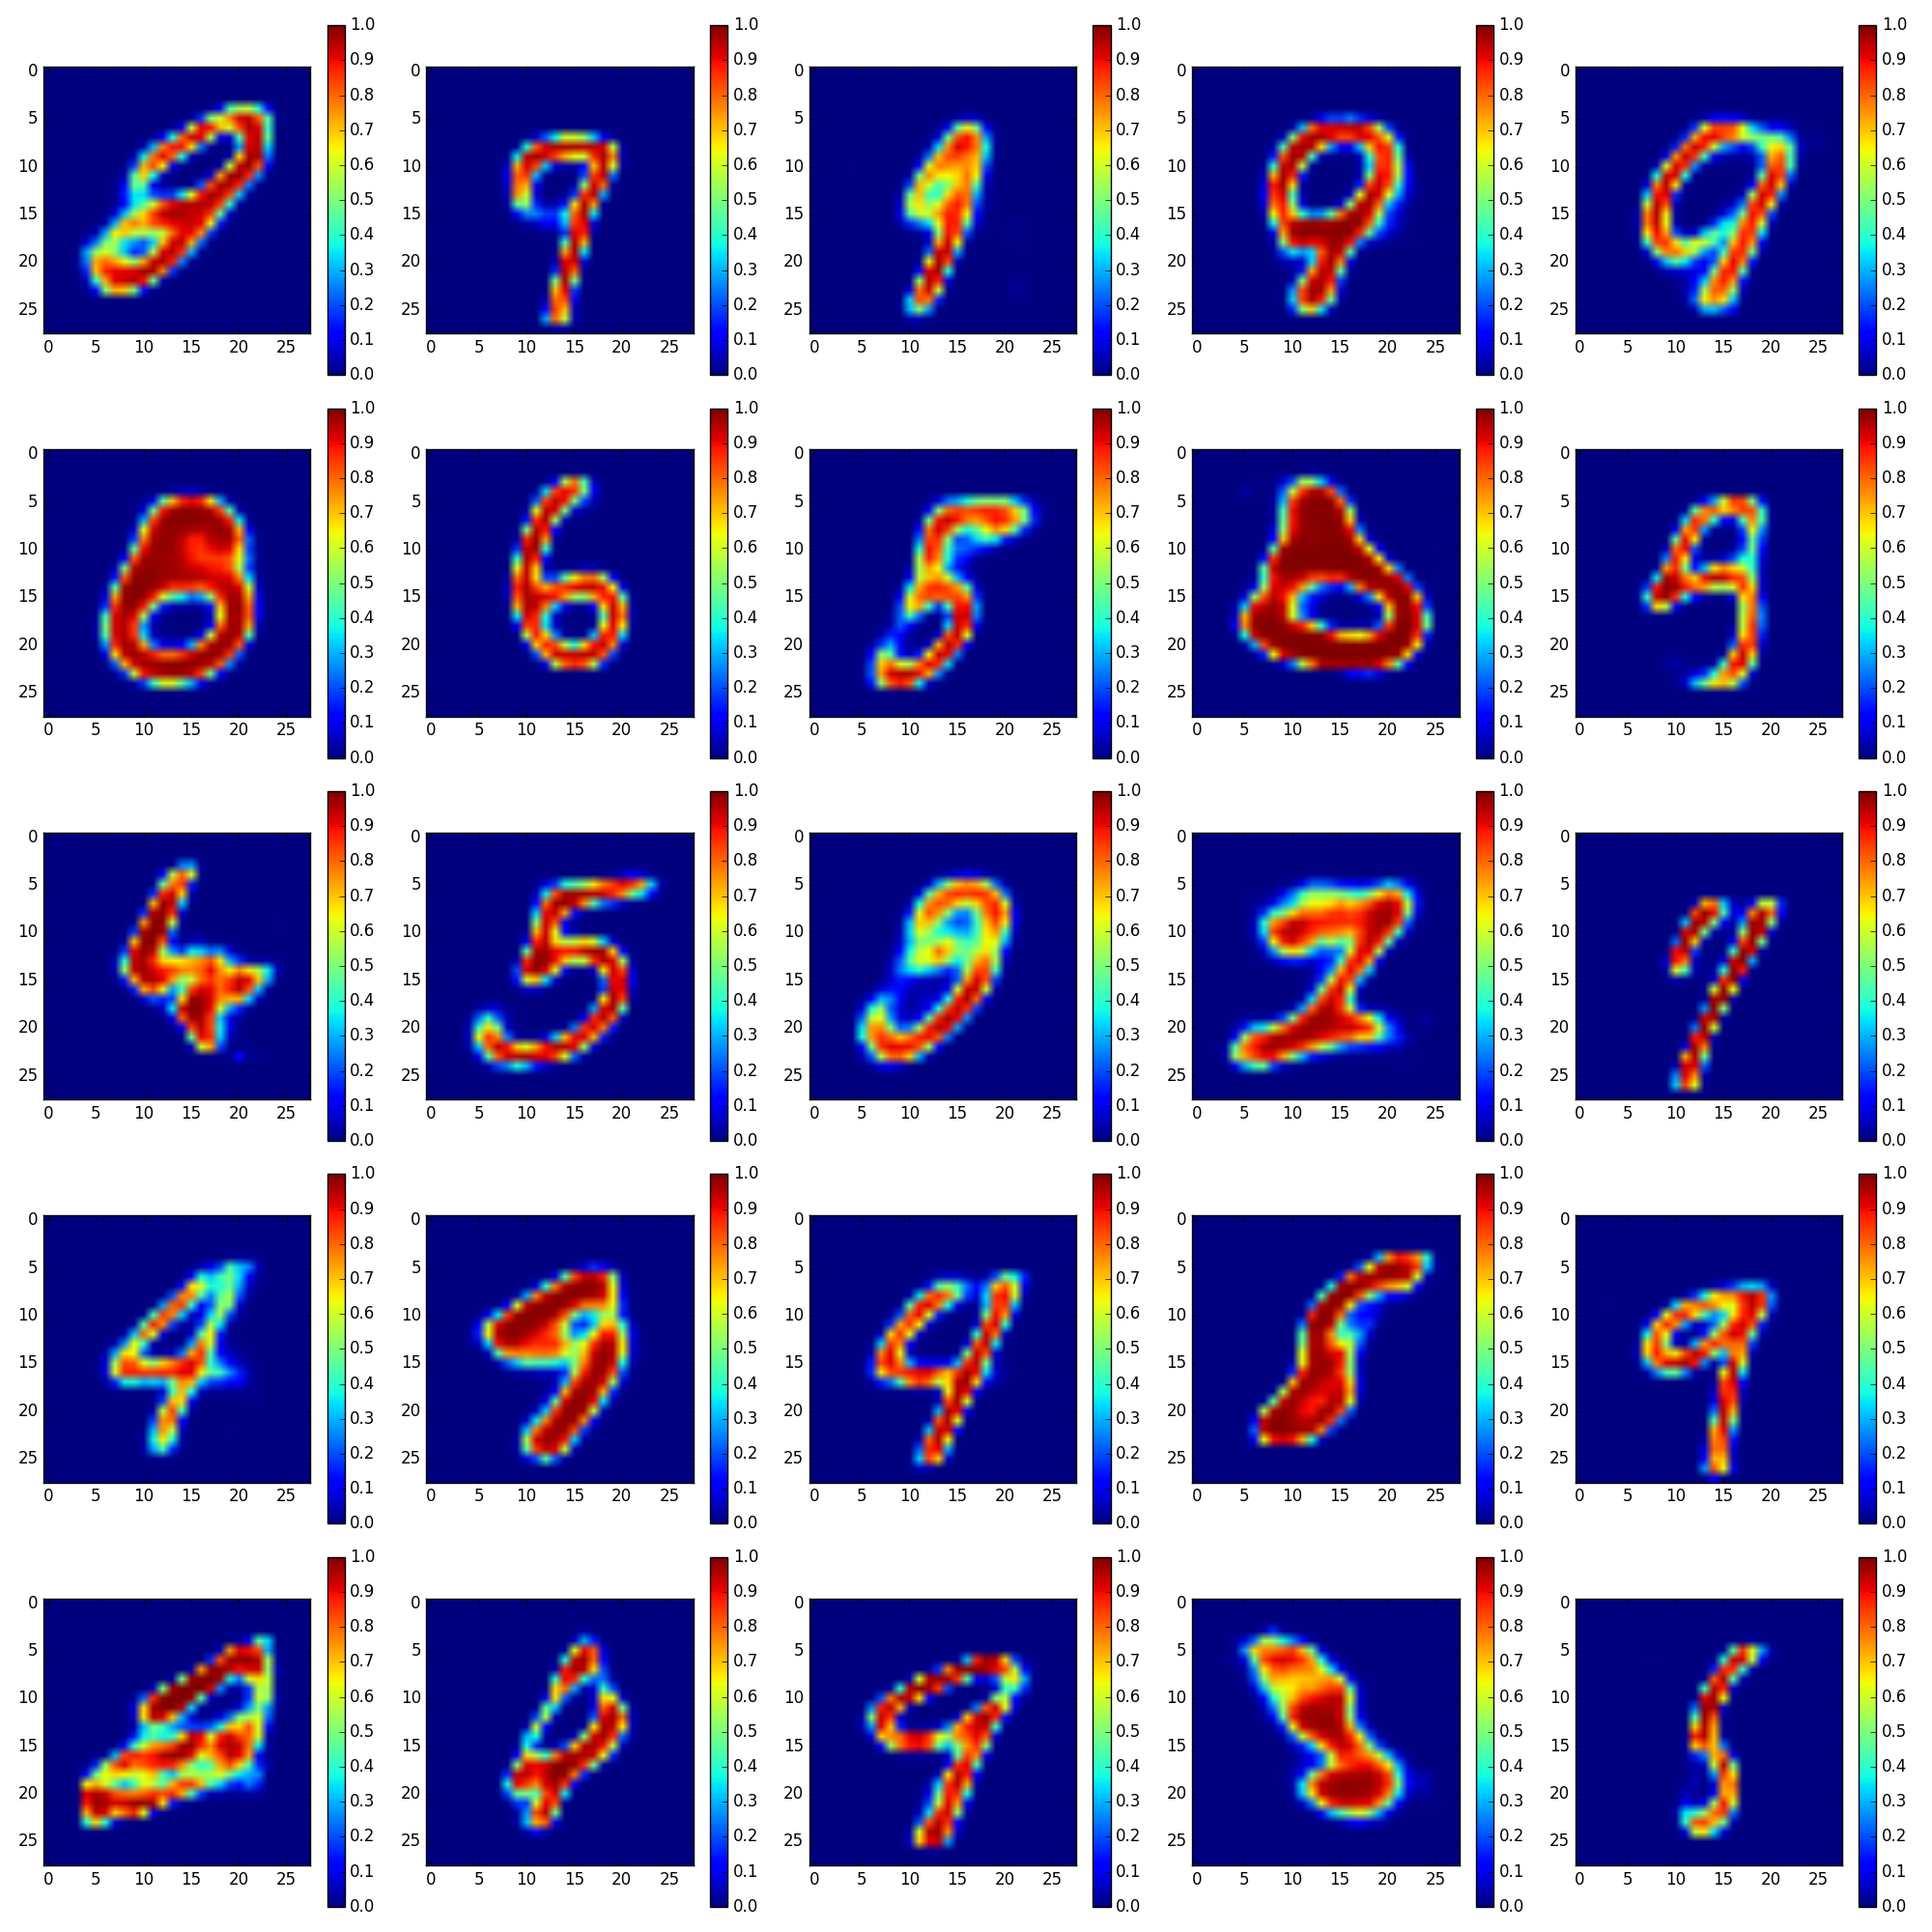
\includegraphics[width=0.4\textwidth]{img/fcvae.png}
        \caption{Output of fc-VAE (left) and conv-VAE (right)}
    \end{figure}
    \item \emph{Conditional VAE (CVAE).} We followed the model described in \cite{doersch2016tutorial}, with fully-connected networks, which essentially is the same as the vanilla VAE, but also takes side information such as partial images or labels. Below we show that, given half of an image, it is able to generate an image that matches the given half. A similar model is able to take a label and generate the corresponding digit, with varying styles.
    \begin{figure}[!ht]
    \centering
    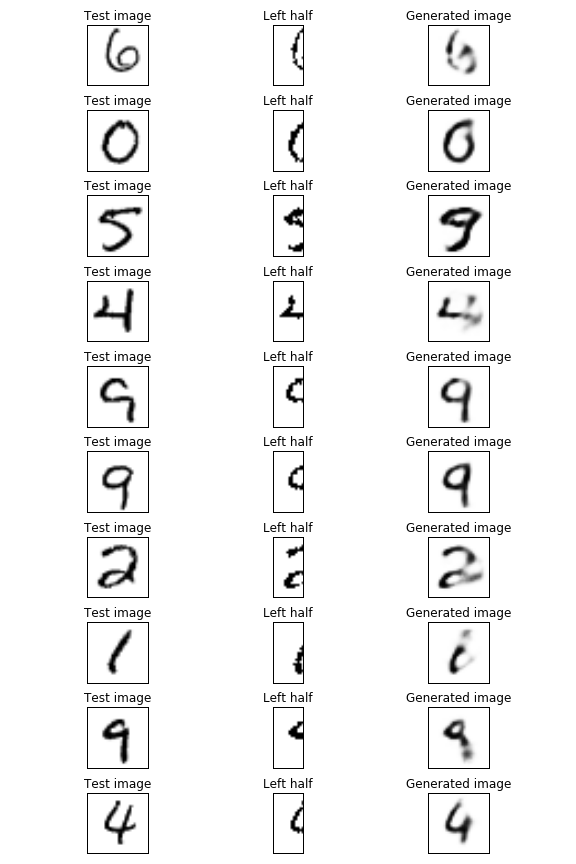
\includegraphics[width=0.4\textwidth]{img/left_half.png}\quad
    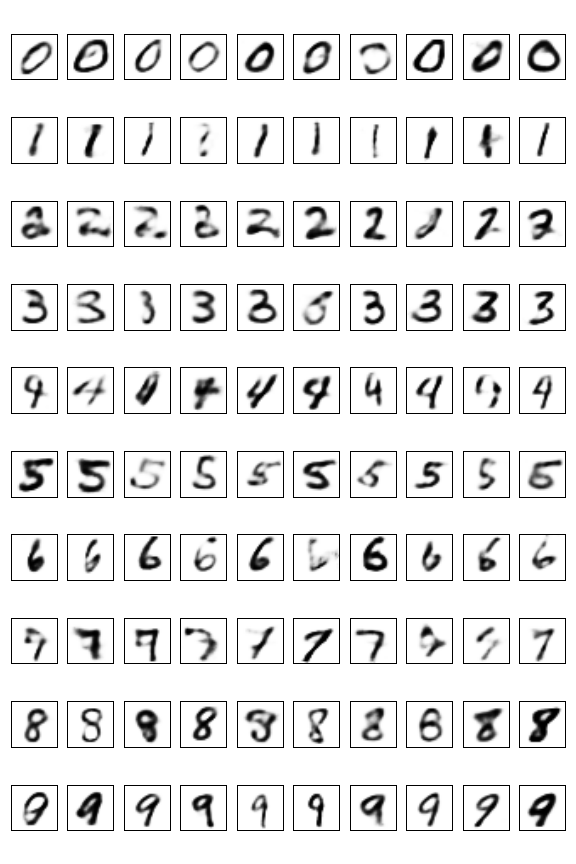
\includegraphics[width=0.4\textwidth]{img/by_label.png}
    \caption{CVAE: Completing half of an image (left), and generating given labels (right)}
    \end{figure}
    \item \emph{DRAW.} This model is based on \cite{gregor2015draw}. The baseline model is a two-LSTM network: the first LSTM is a encoder, which takes an image as input and outputs a low-dimensional vector $z$. The second LSTM is a decoder, with takes $z$ as an input and outputs an image.
    \item \emph{Semi-supervised model.} This model is from \cite{DBLP:journals/corr/KingmaRMW14}. It is slightly more versatile than the CVAE in that it can simultaneously learn from a dataset where not all examples are labeled. We are still setting this up.


\end{enumerate}

\section*{Challenges}

At first we thought replacing fully connected layers with convolutional and deconvolutional layers will improve the results. But then we found it was not the case. Currently the simplest VAE yields the best results with the chosen parameters. We are still tuning the parameters and try to find out whether it is the problem of conv-VAE itself or it is because we select a bad set of parameters.

Implementing the semi-supervised model of \cite{DBLP:journals/corr/KingmaRMW14} was a little tricky because we need to handle labeled and unlabeled data differently.

In all models we still need to find good architectures and tune hyperparameters.



\section*{Tools and related challenges}
We are currently using TensorFlow and collaborating with Github.

When we run our experiments on AWS machines, we only receive the final states of the checkpoint. This makes it hard to tune the parameters. Currently we are adding TensorFlow functions to our code that can report the loss history (in our case we report the encoder loss and decoder loss separately).

The checkpoint files are very large (100-200 MB). Therefore it is difficult to download and upload those files. Further, the naming of the checkpoint files is important. We need to make a consistent rule to name those files when doing experiment separately.

\section*{Evaluation}

Since we are in the nascent stages of our project, we are currently just using eyesight to judge the quality of our generated images. In the future, we may consider other measures such as log-likelihood, or adopt an adversarial approach by applying a discriminator/classifier on our images.

\bibliographystyle{plain}
\bibliography{cs294_bib}

\nocite{*}

\end{document}
